\documentclass{article}
\usepackage[utf8]{inputenc}
\usepackage[spanish]{babel}
\usepackage{ifpdf}
\usepackage{subcaption}
\usepackage{graphicx}
\usepackage{hyperref}
\title{Operación y Mantenimiento de Equipos e Instalaciones Eléctricas Aeronáuticas}
\author{Leandro Marsó}
\date{2015}
\ifpdf
\hypersetup{
    pdfauthor={Leandro Marsó},
    pdftitle={Operación y Mantenimiento de Equipos e Instalaciones Eléctricas Aeronáuticas},
}
\fi

% Para cambiar los nombres por defecto:
% Babel traducía table como cuadro. Yo lo cambio para tabla:
\addto\indexspanish{%
  \renewcommand{\indexname}%
    {Programa de la materia}%
}

\begin{document}
\maketitle
\pagebreak
\tableofcontents
\pagebreak

%Trimestre 1
\section{Electromagnetismo}
\subsection{Introducción}

La fuerza eléctrica y la fuerza magnética son dos fenómenos que se fueron descubriendo y aislando como si fueran dos fuerzas independientes una de la otra, pero la realidad es que son manifestaciones de una única fuerza que se llama fuerza electromagnética. Esta fuerza es la causante de casi todos los fenómenos que experimentamos en el día a día, con excepción de la gravedad. Por ejemplo, cuando empujamos o tiramos de algún objeto, experimentamos el resultado de la interacción entre las moléculas de nuestro cuerpo, con las del objeto que tocamos. Esto se debe a que los núcleos de los átomos y los electrones dentro y alrededor del átomo interaccionan por medio de la fuerza electromagnética. Los fenómenos químicos también son el resultado de la fuerza electromagnética.

\subsection{Fuerza Electromagnética}
Originalmente se pensaba que la fuerza eléctrica y la fuerza magnética eran dos fuerzas separadas, hasta que James Clerk Maxwell realizó la publicación de \emph{Un tratado de electricidad y electromagnetismo} en el que se mostraba que las interacciones entre cargas negativas y positivas estaban reguladas por una sola fuerza.

Existen cuatro efectos principales que son el resultado de estas interacciones, los cuales se pueden demostrar por medio de experimentos:

\begin{enumerate}
\item Las cargas eléctricas se atraen o repelen una a la otra con una fuerza inversamente proporcional al cuadrado de la distancia entre ellas: Cargas de igual signo se repelen, cargas de distinto signo se atraen.
\item Los polos magnéticos se atraen o repelen de la misma forma, y siempre vienen de a pares: Cada polo sur está unido a un polo norte.
\item Una corriente eléctrica en un cable crea un campo magnético alrededor del cable, y su dirección (en sentido horario o anti horario) depende del sentido de esta corriente.
\item Una corriente es inducida en una espira de cable cuando se acerca o aleja a un campo magnético, o un imán se le acerca o aleja a la espira. La dirección de esta corriente inducida depende de la dirección del movimiento del campo magnético.
\end{enumerate}

\subsection{Acción recíproca entre campo magnético y corriente eléctrica}
La corriente eléctrica es el resultado del movimiento neto de cargas a lo largo de un conductor. Por lo tanto, para estas cargas en movimiento podemos decir que se cumple: 
\begin{itemize}

\item Una partícula cargada y en movimiento, creará un campo magnético en sus proximidades.
\item Una partícula con carga eléctrica que se encuentra en movimiento y atraviesa un campo magnético, sufrirá una fuerza debido a la existencia de este campo.

\end{itemize}

Veremos ahora ejemplos de estos fenómenos que acabamos de describir:

\subsubsection{Campos magnéticos creados por corrientes eléctricas.}
El campo magnético que se crea a causa de una corriente eléctrica tiene la forma de la figura \ref{fig:campo}:

\begin{center}
	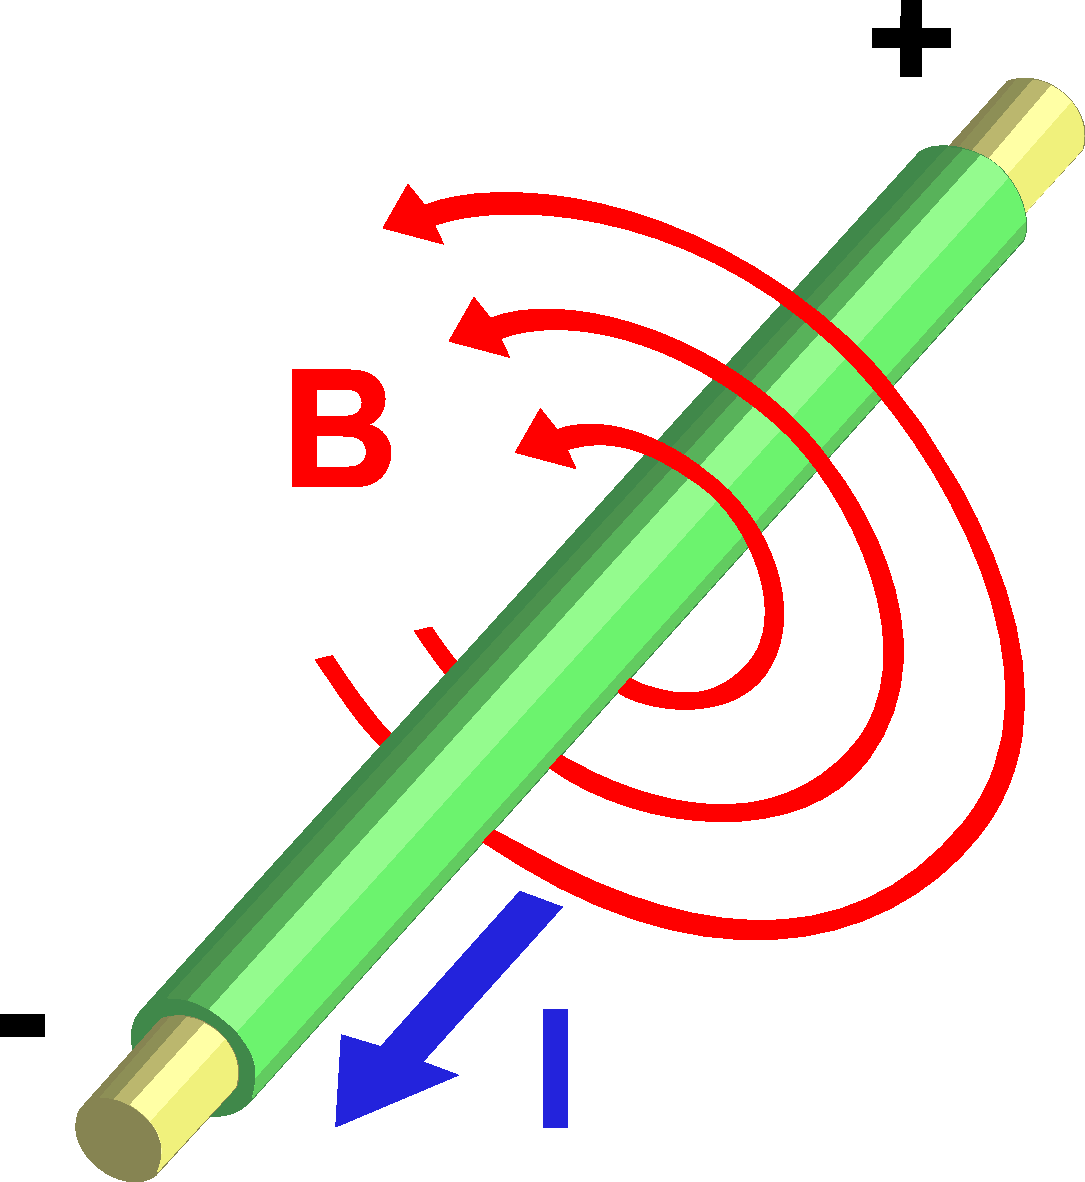
\includegraphics[scale=0.30]{figuras/corriente-campo.pdf}
	\captionof{figure}{\emph{Campo magnético creado por una corriente eléctrica}}
\label{fig:campo}
\end{center}
Podemos utilizar una regla mnemotécnica para saber en que sentido se crea ese campo, a partir del sentido de la corriente. Esta se conoce como la \textbf{regla de la mano derecha}:
\begin{center}
	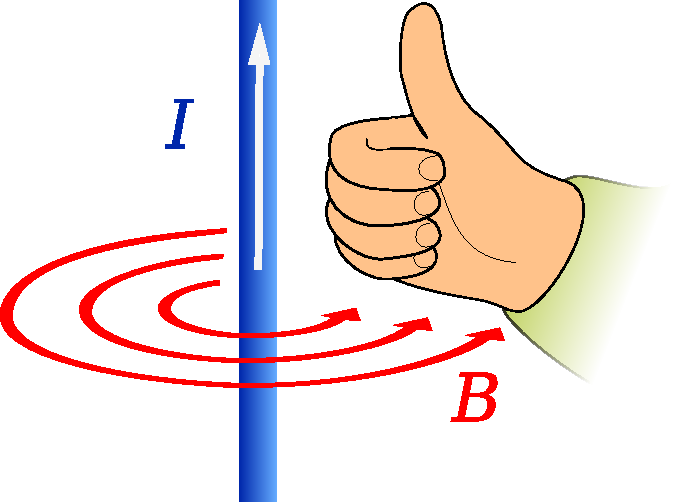
\includegraphics[scale=0.450]{figuras/corriente-campo-reglamano.pdf}
	\captionof{figure}{\emph{Regla de la mano derecha, nos permite recordar el sentido del campo magnético creado por la corriente}}
\label{fig:regla}
\end{center}

Veamos una aplicación de este fenómeno: Si enrollamos un cable como se muestra en la figura \ref{fig:solenoide}, y generamos una corriente eléctrica contínua, lograremos un electroimán. Esta forma de enrollar el cable se llama forma de solenoide.
\begin{center}
	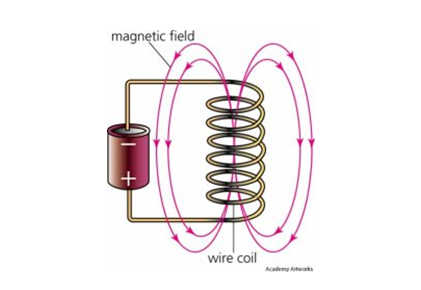
\includegraphics[scale=0.50]{figuras/electroiman-3.png}
	\captionof{figure}{\emph{Electroimán}}
\label{fig:solenoide}
\end{center}
Para entender el resultado, veamos en detalle qué pasa con el campo magnético creado por la corriente, cuando la misma circula por las espiras de este solenoide:
\begin{center}
	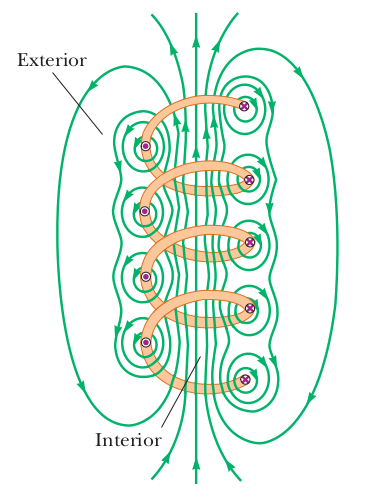
\includegraphics[scale=0.50]{figuras/solenoide-1.png}
	\captionof{figure}{\emph{El círculo con punto indica que la corriente entra desde atras del plano del papel, y el círculo con cruz indica que la corriente cruza saliendo hacia atras del plano del papel.}}
\label{fig:solenoide-1}
\end{center}

Si el solenoide tiene las espiras bien juntas una a la otra, se logra un electroimán con un campo magnético muy uniforme dentro del solenoide y externamente muy parecido a un imán, como se puede ver en la figura \ref{fig:solenoide-2}.
\begin{center}
	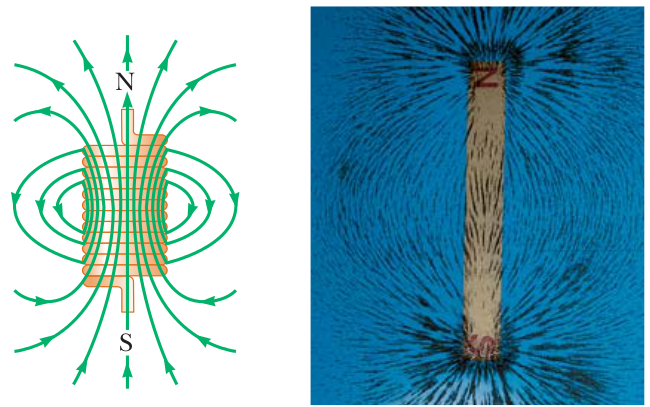
\includegraphics[scale=0.50]{figuras/solenoide-2.png}
	\captionof{figure}{\emph{ Observe que las líneas de campo se parecen a las que existen alrededor de un imán de barra, lo que significa que efectivamente el solenoide tiene polos norte y sur. En la figura de la derecha se puede observar el patrón del campo magnético de un imán de barra, desplegadas mediante limaduras de hierro sobre una hoja de papel}}
\label{fig:solenoide-2}
\end{center}


%\subsubsection{Movimiento de una partícula con carga en un campo magnético uniforme} % Regla de la mano izquierda 
\subsubsection{Campo magnético unifirme sobre un conductor que transporta corriente} 

En un conductor que está dentro de un campo magnético perpendicular a él y por el cual se hace circular una corriente, se crea una fuerza cuyo sentido dependerá de cómo interactúen ambas magnitudes (corriente y campo). Para obtener el sentido de la fuerza, se toma el dedo índice de la mano (izquierda) apuntando a la dirección del campo magnético que interactúa con el conductor y con el dedo medio se apunta en dirección a la corriente que circula por el conductor, formando un ángulo de 90 grados. De esta manera, el dedo pulgar determina el sentido de la fuerza que experimentará ese conductor.


\begin{center}
	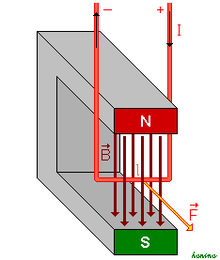
\includegraphics[scale=0.99]{figuras/corriente-campo-fuerza.png}
	\captionof{figure}{\emph{Fuerza que actúa sobre un conductor que transporta corriente, con la regla de la mano izquierda se puede conocer el sentido de esta fuerza.}}
\label{fig:corriente-campo-fuerza}
\end{center}

Veamos otro gráfico con el mismo efecto:

\begin{center}
	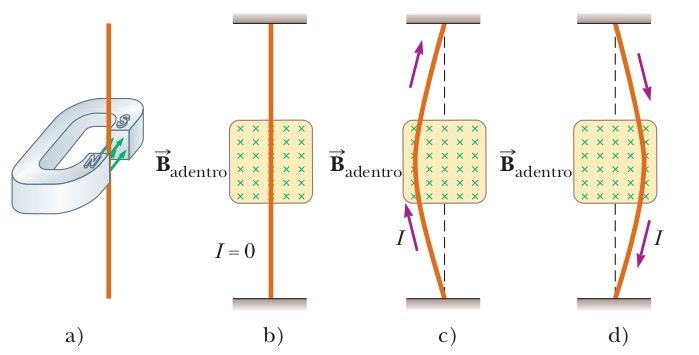
\includegraphics[scale=0.51]{figuras/corriente-campo-fuerza-2.png}
	\captionof{figure}{\emph{a) Imán que genera el campo magnético y la ubicación para realizar el experimento. b) Vemos el conductor y de fondo el polo sur del imán, líneas de campo representadas con las cruces. c) La corriente en un sentido genera una fuerza que mueve el cable hacia la izquierda. d) La corriente en el sentido inverso en presencia del mismo campo, genera una fuerza hacia el otro lado. }}
\label{fig:corriente-campo-fuerza-2}
\end{center}



%\subsubsection{Fuerza que actúa sobre un conductor que transporta corriente}


%Trimestre 2
\pagebreak
\section{Corriente Alterna }

%Trimestre 3
\section{Resolución de circuitos en corriente alterna}



\end{document}
